\documentclass[a4paper,12pt]{report}

\newcommand{\firstauthor}{Jorge Erustes}
\newcommand{\secondauthor}{Oier Saizar}
\newcommand{\thirdauthor}{Ainhoa Ach\'on}
\newcommand{\fourthauthor}{Alejandro Mart\'in}
%\newcommand{\groupnumber}{}
\newcommand{\docversion}{Version 3.59}

% include packages
\usepackage[margin=2cm]{geometry}
% \usepackage{color}
\usepackage{xcolor}
\usepackage{graphicx}
\usepackage{subfigure}
\usepackage{booktabs}
\usepackage{parskip}
\usepackage[pdftex]{hyperref}
\usepackage[titletoc]{appendix} % adds ``Appendix'' prefix in TOC
\usepackage{listings}
\usepackage{url}
\usepackage{csquotes}

\definecolor{keyword}{HTML}{B71C1C}
\definecolor{foreground}{HTML}{000000}
\definecolor{background}{HTML}{FFFFFF}
\definecolor{codecomment}{HTML}{757575}
\definecolor{identifier}{HTML}{0D47A1}
\definecolor{mymauve}{rgb}{0.58,0,0.82}

\graphicspath{ {images/} }

% configure packages
\lstset{language=bash,
    basicstyle=\footnotesize\ttfamily\color{foreground},
    frame=single,
    breaklines=true,
    columns=fullflexible,
    keepspaces=true,
    numbers=left,
    numberstyle=\tiny,
    stepnumber=2,
    numbersep=5pt,
    identifierstyle=\color{foreground},
    keywordstyle=\color{foreground},
    rulecolor=\color{foreground},
    stringstyle=\color{mymauve},
    commentstyle=\color{codecomment},
    backgroundcolor=\color{background}
    }

% pdflatex goodies.
\hypersetup{
    pdfstartview=FitH,
    pdftitle={DaaS},
    pdfauthor={\firstauthor, \secondauthor, \thirdauthor, \fourthauthor},
    pdfsubject={},
    pdfkeywords={ansible, openstack, d&d}
    bookmarks,
    bookmarksopen,
    colorlinks,
    linkcolor=black,
    citecolor=blue,
    urlcolor=blue,
}

\newcommand{\TODO}[1]{\textcolor{red}{\newline TODO: #1}}


\title{{\Huge\textbf{Dungeons\&Dragons as a Service}}}
\author{\Large \firstauthor\\\Large \secondauthor\\\thirdauthor\\\fourthauthor\\\mbox{}\\\mbox{}\\\docversion}
\date{\today}

\setlength{\parindent}{0cm}

\begin{document}

\renewcommand{\thepage}{\roman{page}}
\maketitle
\tableofcontents
\addcontentsline{toc}{chapter}{Table of Contents}

\chapter{Introduction}
\setcounter{page}{1}
\renewcommand{\thepage}{\arabic{page}}

Dungeons \& Dragons as a Service is born to pave the way for fast and automated 21st-century role-game campaign creation and configuration. DaaS works as a framework in which one can quickly start playing D\&D in a Cloud instance automatically launched by the service, already configured for a \textit{launch-and-play} experience. 

All participants can choose the details of their characters through a Web-Server wizard, guiding them through the process, including class, stats and race selection. Once chosen, DaaS takes charge of the rest and ensures a Cloud instance is created, in which the characters are setup for login for the users and Dungeon Master to do so. When logging in, characters will find the access to their spells already configured. All spell access will be based on the character's level and class, as there will be an Access Control List running to make sure each character is limited to their legitimate capabilities.

The Web Server runs in an Apache Server, and uses Ansible to tell the machine in charge of the instances (CentOS) to launch a new instance to host the new campaign. This Cloud Campaign will be a CentOS as well, which will be remotely configured via Ansible with everything necessary for the game to go smoothly. Spells are organized as files in a file tree separating character classes and levels while these spells' permissions to be used are remotely configured too through an Access Control list based on the character's attributes.



%%%%%%
\chapter{Planning}
\label{ch:plan}

During this chapter we will cover everything regarding the structure of the whole infrastructure. This will include all technological and logical details of how the service is thought and planned out.

The basic structure of the service will be sketched out below and will consist of the following.
\begin{itemize}
    \item \textbf{Clients}: These represent the user machines, through which they connect to the service to create the campaign, choose their characters and later connect to the Cloud Campaign instance.
    \item \textbf{WebServer}: This Debian machine is in charge of serving as a crossroads for user interaction and instance configuration, as will be seen later in greater detail. Uses a mySQL database.
    \item \textbf{RDO (OpenStack Server}: This CentOS machine is in charge of the Cloud Instance creation and configuration. It uses OpenStack to do so, and will be referred to as RDO from now on.
    \item \textbf{Cloud Campaign}: These are the Cloud Instances in which the campaigns are hosted, running on Ubuntu machines and launched from RDO.
\end{itemize}

\begin{figure}[h!]
\caption{Diagram of machines taking part in the service.}
\centering
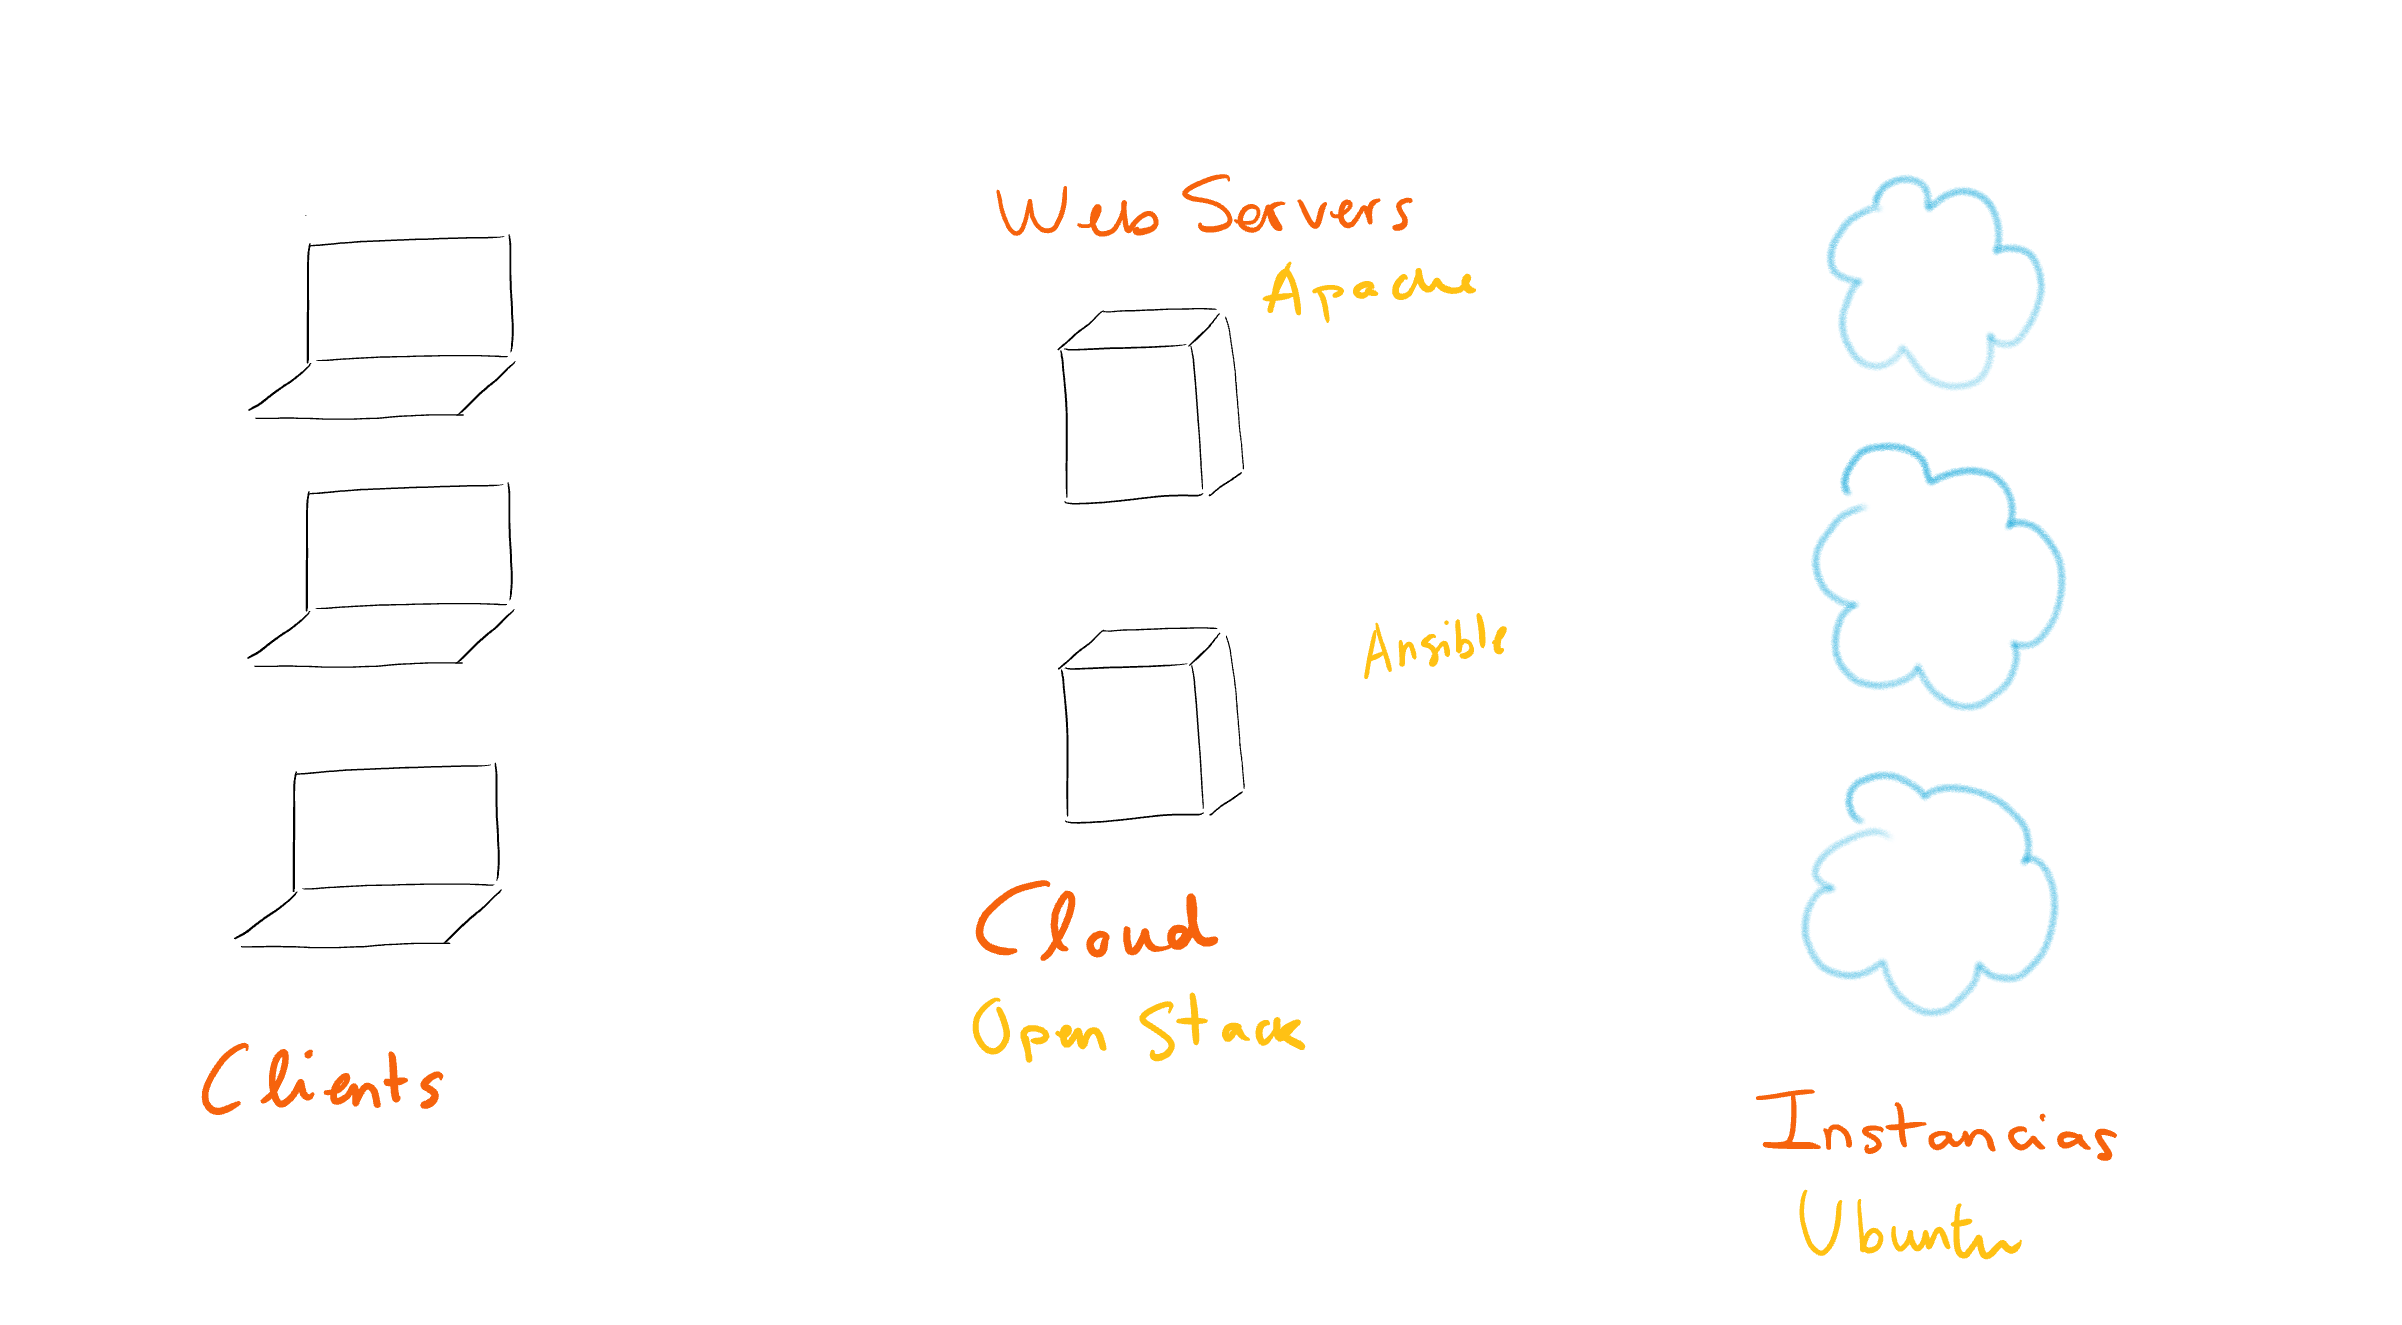
\includegraphics[width=0.75\textwidth]{images/Capture1.PNG}
\label{fig:diagram1}
\end{figure}



    %%%
\section{Web Server and Ansible}
\label{sec:planWS}
The Web Server is deployed as a web application using the Flask micro-framework (Python) running over a mySQL database.
This server is in charge of Ansible to set up the remote configuration of the rest of the system.

Ansible has two main tasks in the service: 
\begin{itemize}
    \item \textbf{Order Cloud Instance creation}: The server will task the RDO (OpenStack Server) the creation of Cloud Instances which will host the game campaigns, using Ansible as communication. The Web Server sends an Ansible script to the RDO, who will use it together with OpenStack to launch these Cloud Campaign instances. In this instance, a file system has already been established which will set as the foundation for the system behavior to be explained during this section. Details on such file system can be found in \autoref{sec:planDir}.

    \item \textbf{Remote Configuration of Instances}: Once the Cloud Campaigns are up, the Web Server launches Ansible to configure these instances. 
    \begin{enumerate}
        \item \textit{Group creation}: Linux groups are created in the remote Linux instances (Cloud Campaigns). These groups are of two types: Character Classes (Warlock, Wizard, Paladin...) and Level (0, 1,.. 9). They will be used to place the playing characters in them according to their Class choice and Level (0 by default at Campaign Opening). 
        \item \textit{Character creation}: With the registered user's characters, Ansible is used to create new users in the Cloud Campaigns, belonging to the groups: Class\_name \& 0 (character level). The choice made when configuring the campaign in the Web Server will determine which Class are they placed into, and they start at Level 0 with their characters.
        \item \textit{Permission Setting}: In order to correctly configure what Spells can each character use, we employ Ansible to set up an Access Control List on the Spell files to ensure no character can access a Spell outside of its range (other Class different than its own or Level higher than its current one). The logic behind the Access Control will be detailed further in upcoming sections.
    \end{enumerate}
\end{itemize}



    %%%
\section{Directories}
\label{sec:planDir}

When a Cloud Campaign is created, it contains a set of folders and files representing the Spells available to each Class/Level. To represent this, we have organized these files as follows:
\begin{itemize}
    \item All of the files will be stored on the \enquote{/opt/} directory
    \item This directory holds two sub-directories:
    \begin{itemize}
        \item \enquote{/opt/sp\_lvl/} contains all of the available spells organized in folders depending on their level
        \begin{itemize}
            \item e.g. The level 0 spell \enquote{Eldritch Blast} is in \enquote{/opt/sp\_lvl/0/Eldritch\_Blast.json}
        \end{itemize}
        
        \item \enquote{/opt/ch\_class/} contains links to all the spells in \enquote{/opt/sp\_lvl/} organized by the classes that can use them and then their level
        \begin{itemize}
            \item e.g. The level 0 Warlock Spell link is in \enquote{/opt/ch\_class/Warlock/0/\\ Eldritch\_Blast.json}
        \end{itemize}
    \end{itemize}
\end{itemize}
We organize Spells in these two different directories because we will create ACLs based on two groups that represent the character's Class and Level.
In order to reduce possible incongruity between one directory and the other, we have decided to create links in one to the files on the other. 

\subsection{Character Creation}
\label{subsec:characterCreation}
When the user logs in for the first time, they will run a Python script to further define their Character's characteristics. The script is a small command line program that will interact with the user, and after fetching the initial data defined on the Web API (Character name and Class), it will add new data like the Character's race or their Ability/Stats. When the script finishes, it will generate a .txt file
containing all the details, as well as the spells this particular character will have access to.


    %%%
\section{Access Control Management}
\label{sec:planACL}
The Access Control system is based on an adaptation of Bell-LaPadula model to the scenario presented in this occasion. From now on, this adapted model, if the reader allows for the authors' literary freedom, will be renamed as \textbf{Bell-LaPseudoPadula}(BLPP).

In the security model present in the Cloud Campaigns, our to-be-secured environment, consists of Linux users (Campaign characters) which belong to Linux groups (roles/attributes in the game, character class and level). Therefore, these groups can be re-interpreted as \textit{security clearance}.
On the other hand, we have Spells, the to-be-regulated object, to which characters aspire to gain access to. These Spells will simply be Linux files in the file system (\textit{json} files), so the restriction of use of such spells in the game logic will translate to confidentiality of such files from users, i.e. whether or not they can read such files based on their Class and Level.

Now it is the point where original Bell-LaPadula come into play. The \textbf{Simple Security Property} (\textit{"no read-up"}) is implanted onto the design of the security model as a subject (Linux user/character) with its respective clearance may not read (have access/use permission) an object (Spell file) at a higher classification (character Level)

The \textbf{*-Property} does not apply as we know it, as no action in the current behavior of the game resembles the \textit{write} action. However, we do have another property taking part in the model. It is what we will, from now on, call the \textbf{Cross Class Property} (CCP). Classes in the role game act as a BLP 'category', and this property will consist of the lack of permission of a character (subject) to access objects (Spell files) belonging to a different Class than its own.

Finally, Bell-LaPadula contains the \textbf{Discretionary Security Policy}, in which an access matrix is used to specify the discretionary access control of objects, what is effectively translated into an AND operator between \textit{SSP} and \textit{*-Property}. Despite some differences and lack of a \textit{*-Property}, our BLPP model retains the DSP property, as we happen to apply an AND operator to our SSP and CCP. This takes effect as a character (user) will lack access (read permission) to a Spell (file) unless his/her Class(es) do encompass that of the target Spell \textbf{AND} its Level is less or equal to that of the character itself.


%//FINAL de este CAPITULO (todo esto tiene que estar explicado)

This configured structure sets an environment where Linux groups are acting as key attributes/ roles for the characters --Linux users-- in order to manage the Spells (i.e. \textit{json} file) they can legitimately access and make use of (i.e. read file), according to the Class choice and level at which they are at.


    %%%
\section{Cloud Instances: Virtualization}
\label{sec:planCloud}

The tool that we have selected to deploy the servers that will host the D\&D games is OpenStack, which is a cloud computing project to provide infrastructure as a service (IaaS). With OpenStack we will be able to deploy as many instances as we wish to play different games just by executing a script.

There are different solutions and distributions of OpenStack in the market, but because of the limited resources available, we have chosen an open source distribution developed by RedHat, called RDO. This distribution allows to install, on a single node (known as \enquote{all-in-one}), all the components and services that compose OpenStack: compute, controller, storage, etc, which are normally deployed on different machines in a distributed way.

Being a RedHat distribution, the libraries to install RDO are available for both Centos and RHEL 7, but not for Debian/Ubuntu-based distributions. 

The modules/components of OpenStack are the following:
\begin{itemize}
\item Dashboard: provides a User Interface accessed via web browser 
\item Compute: it is a controller that manages and hosts the deployed instances. 
\item Network: it is a system for the management of networks and IP addresses.
\item Image: provides discovery, registration and delivery services for disks and the image server. Stored images can be used as a template
\item Storage: Storage System
\item Identity: provides a central directory of users assigned to the OpenStack services they can access
\end{itemize}

%\~napa as a service
\begin{figure}[h!]
\caption{OpenStack components}
\centering
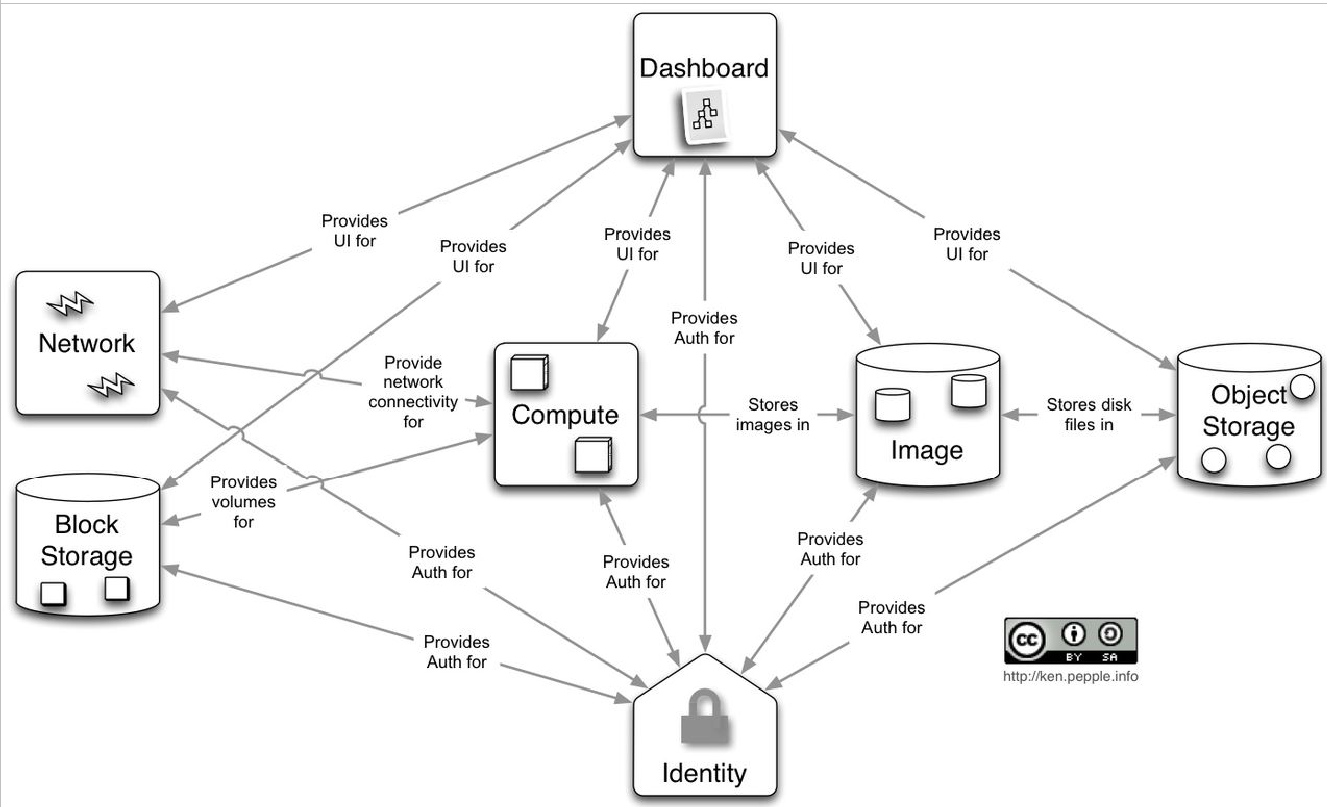
\includegraphics[width=1\textwidth]{images/Selection_101.png}
\label{fig:planVirt}
\end{figure}

\subsection{Deployment}

To deploy the virtualized infrastructure (in this case a server that will host the game) in an automated way, calls will be made to its API rest interface through the use of a script.

This script is developed in Shell bash, and the deployment procedure consists of the following steps:
\begin{itemize}
\item Load through the command \enquote{source} the environment variables to obtain the necessary privileges (user) to be able to deploy the server.
\item Call to the computer service with the definition (characteristics) of the server to be deployed
\item Creation of a floating ip, which is an ip address of the virtual public network created by OpenStack to access the deployed server.
\item Assignment of the floating ip to the deployed virtual machine (instance)
\end{itemize}

Thanks to the use of the tools such as Ansible and OpenStack we have been able to develop a system to deploy virtualized servers easily and quickly using Ansible's own playbooks.

The main advantages of using virtualization technologies are:
\begin{itemize}
\item Ability to monitor and manage network equipment virtualized as if they were physical equipment, with the difference that if changing the configuration of the machine, this becomes unusable or inaccessible would not have to re-install any physical or virtual machine running on any computer, but simply launch the deployment script again.
\item Availability of different network scenarios in a short period of time, only as long as it takes the deployment process to finish. This allows players to have a wide variety of scenarios, and work on different cases of use.
\end{itemize}

%%%%%%
\chapter{Deployment: Use Case}
\label{ch:dev}

Inside this chapter, we will attempt to explain in a more graphical fashion the process of character creation, instance creation and configuration of a Cloud Campaign, precisely the purpose and expected behavior of this DaaS.


We will begin with users of the game connecting to the Web Server to create their character, which is later stored in the database this Server is connected to. This character would consist of just name and Class. [\autoref{fig:UC1}]

\begin{figure}[h!]
\caption{}
\centering
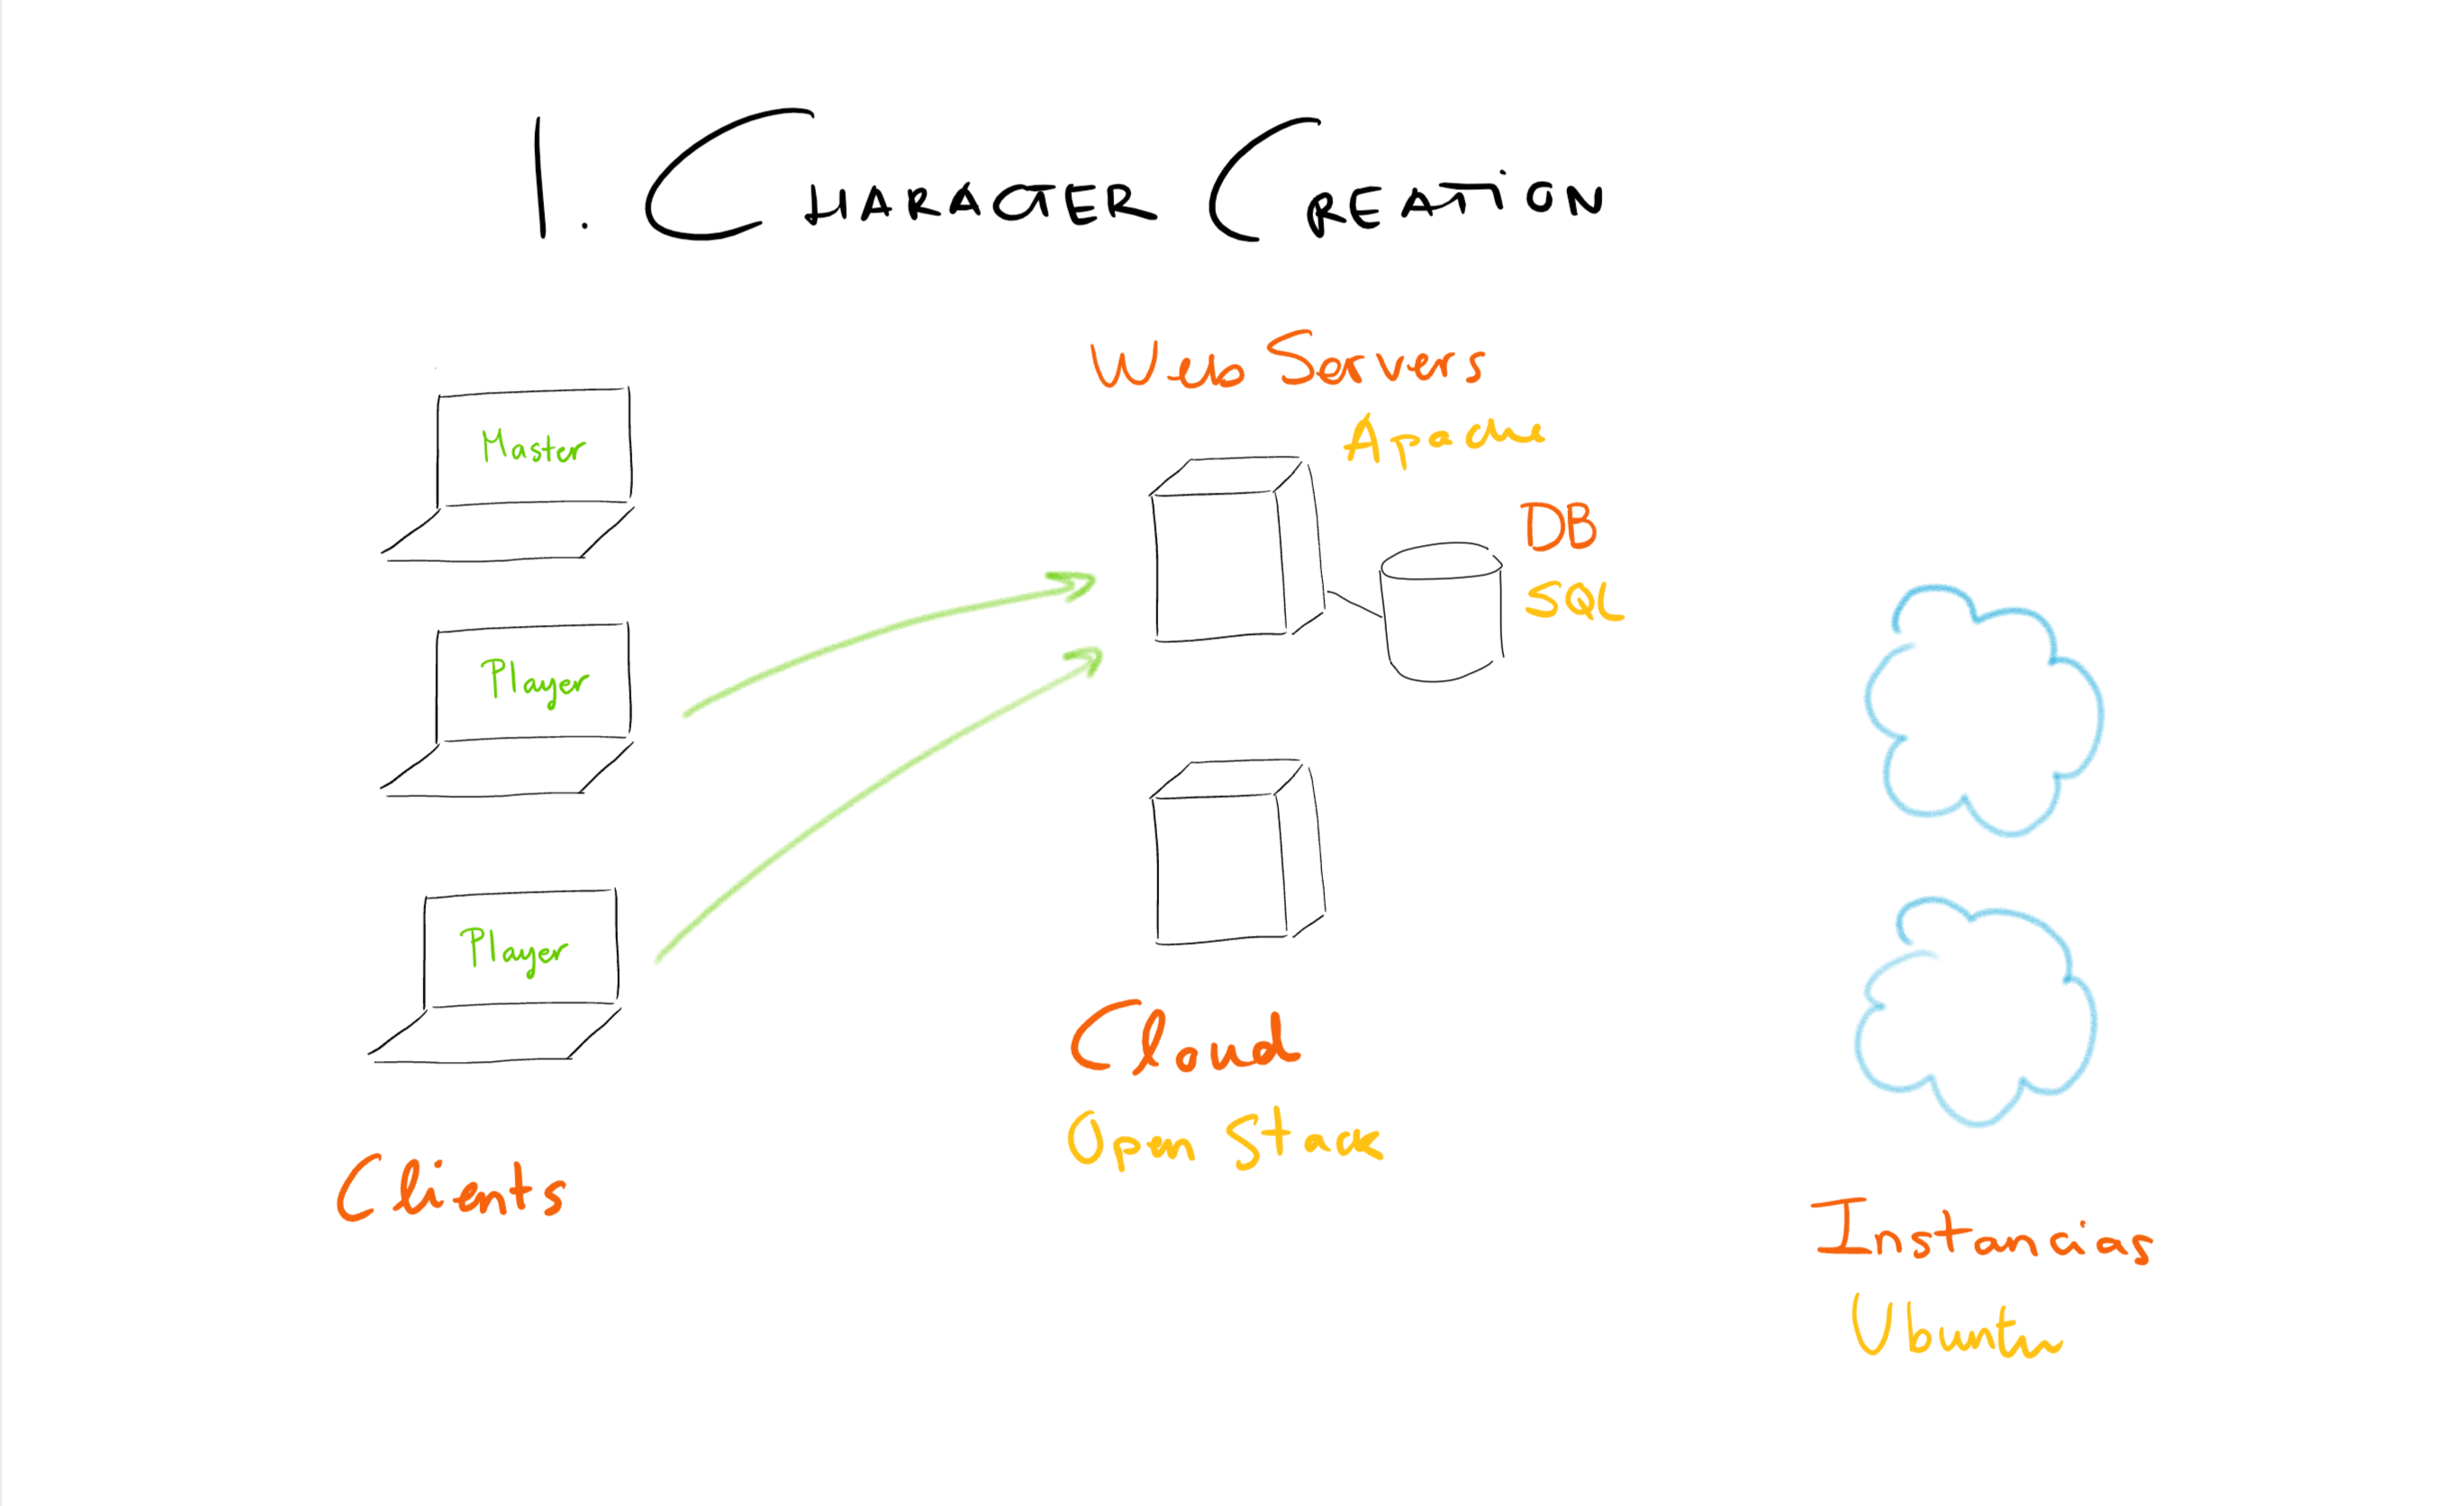
\includegraphics[width=1\textwidth]{images/Phase1.png}
\label{fig:UC1}
\end{figure}


Once characters are created in the Web Server, the Dungeon Master connects to that same Web Server and creates a Campaign with those characters created just before, so they can take part in such Campaign. [\autoref{fig:UC2}]

\begin{figure}[h!]
\caption{}
\centering
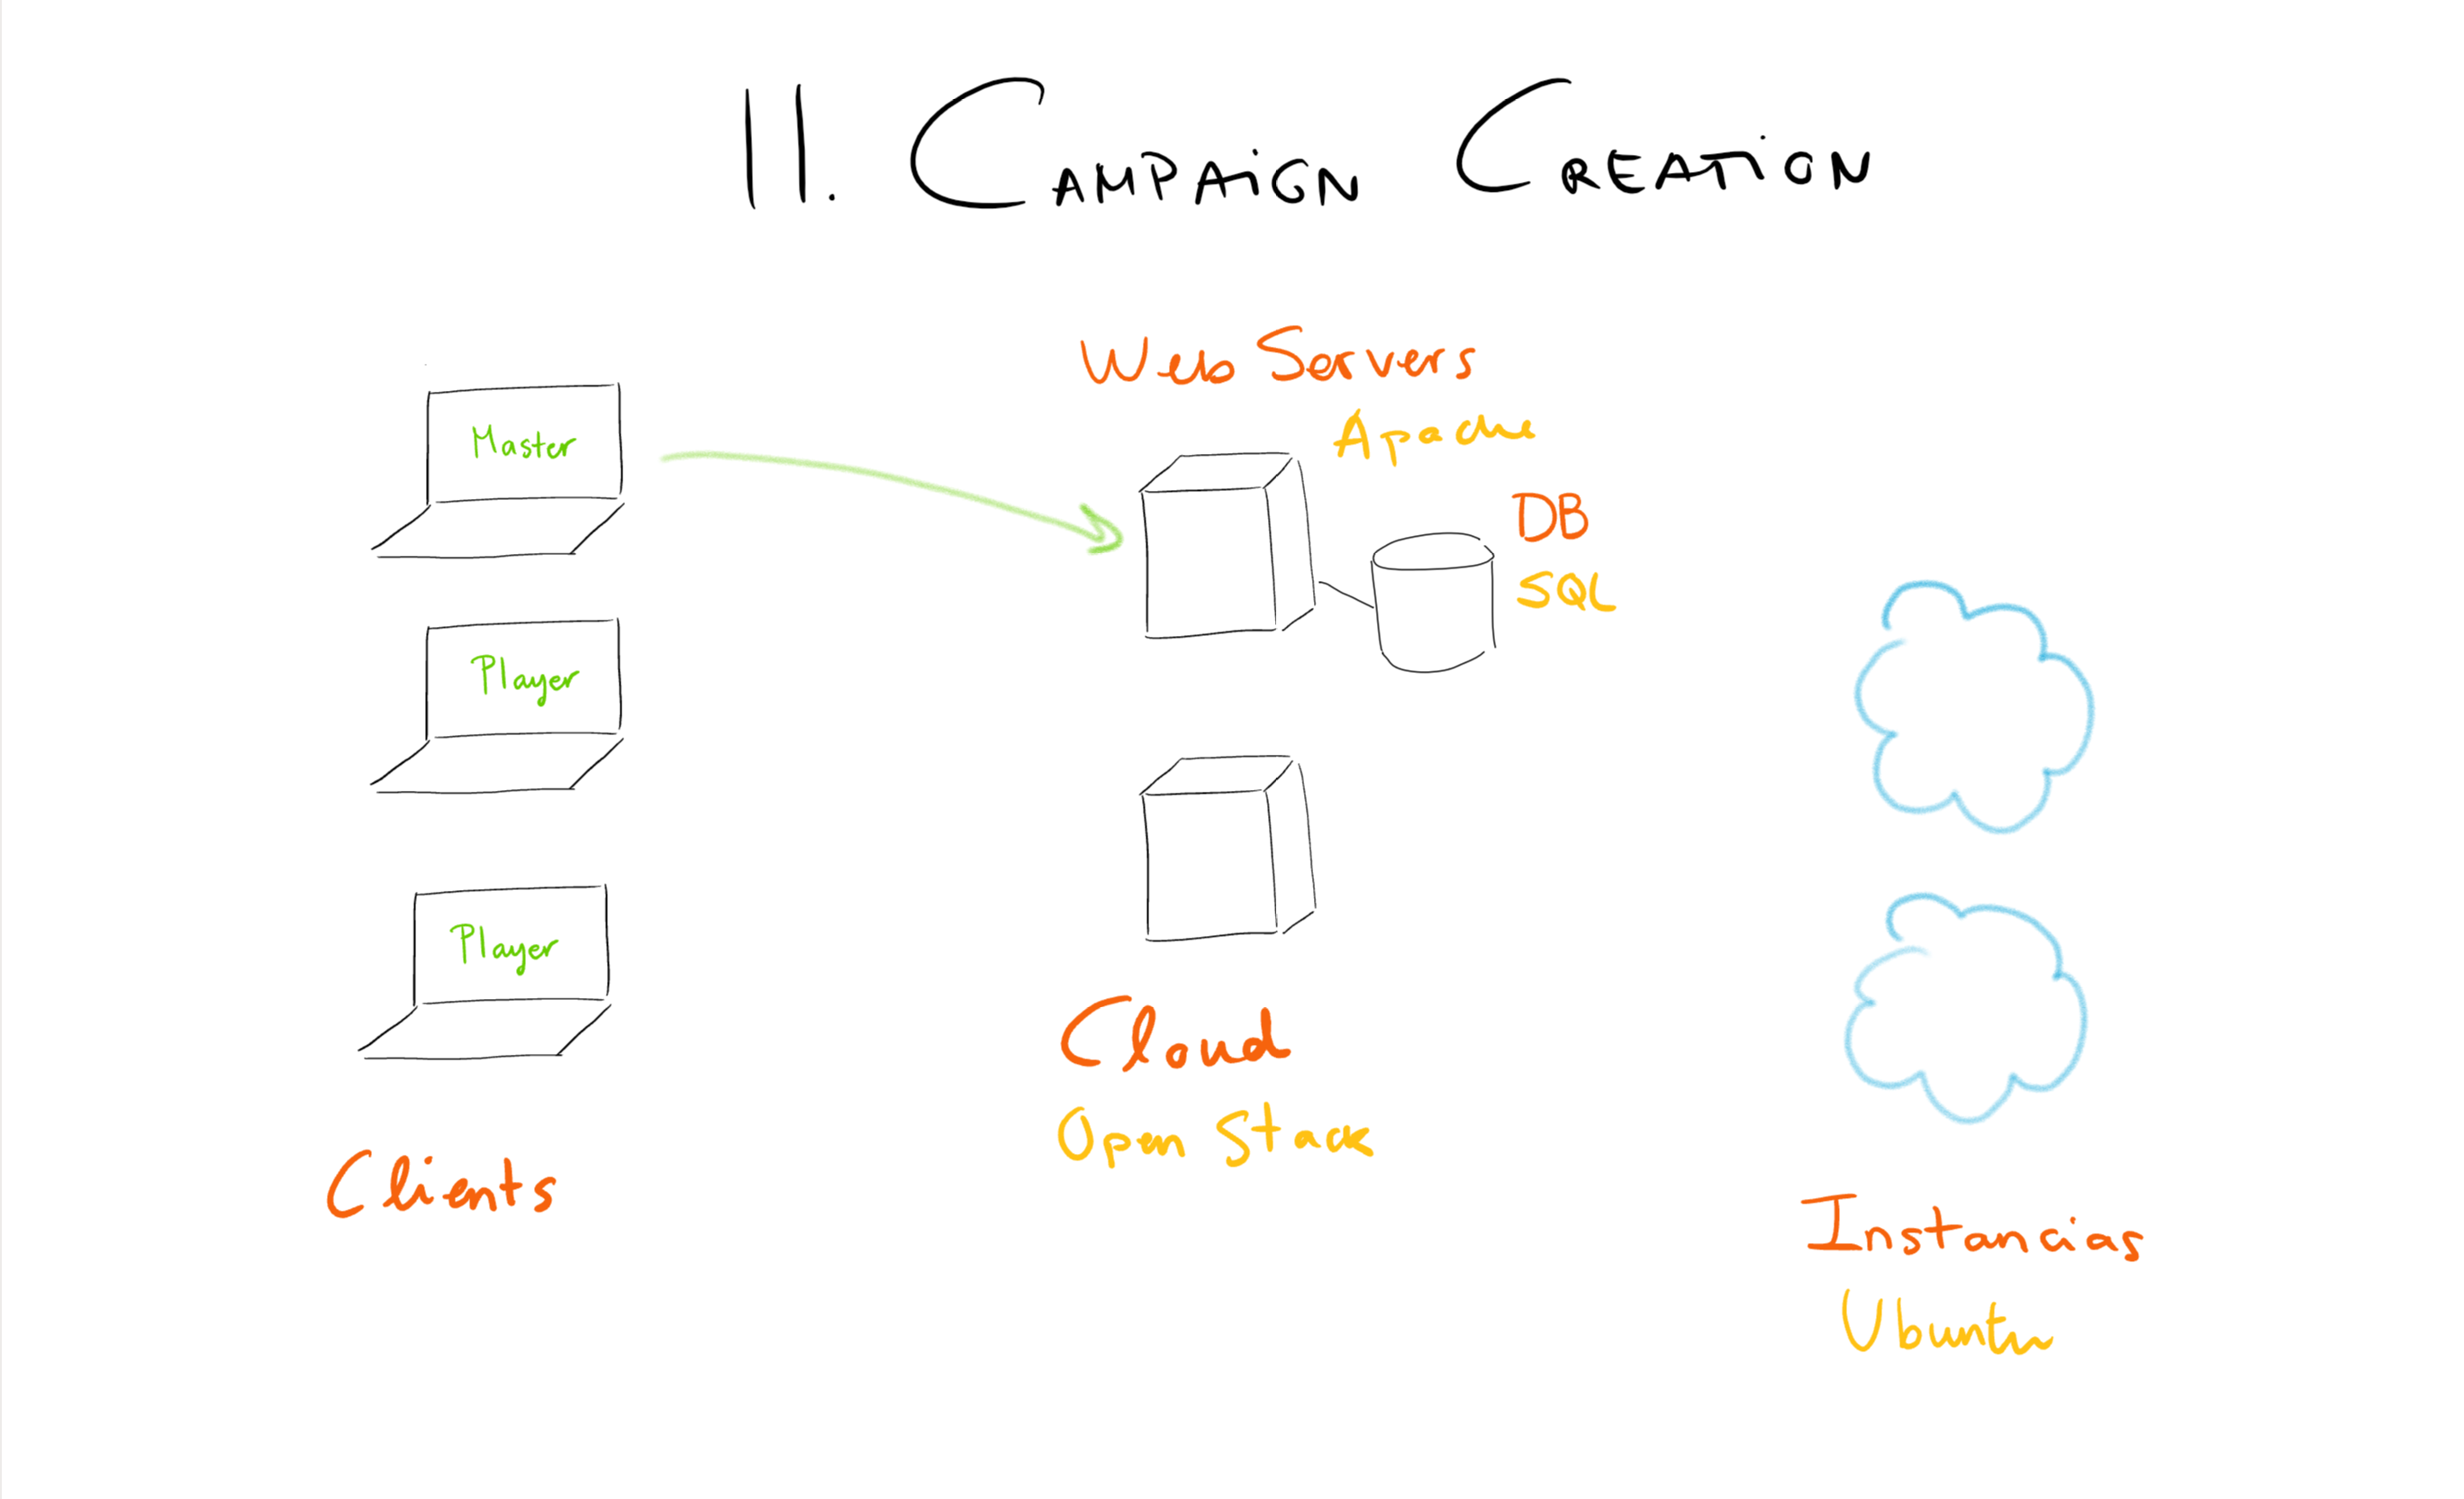
\includegraphics[width=1\textwidth]{images/Phase2.png}
\label{fig:UC2}
\end{figure}


By the time the Campaign has been agreed on by the users, the Web Server starts the Ansible-enabled communication with the Cloud Server, in charge of OpenStack. The goal here would be to order this server to start the creation of the Cloud Campaigns in a remote instance. [\autoref{fig:UC3}]

\begin{figure}[h!]
\caption{}
\centering
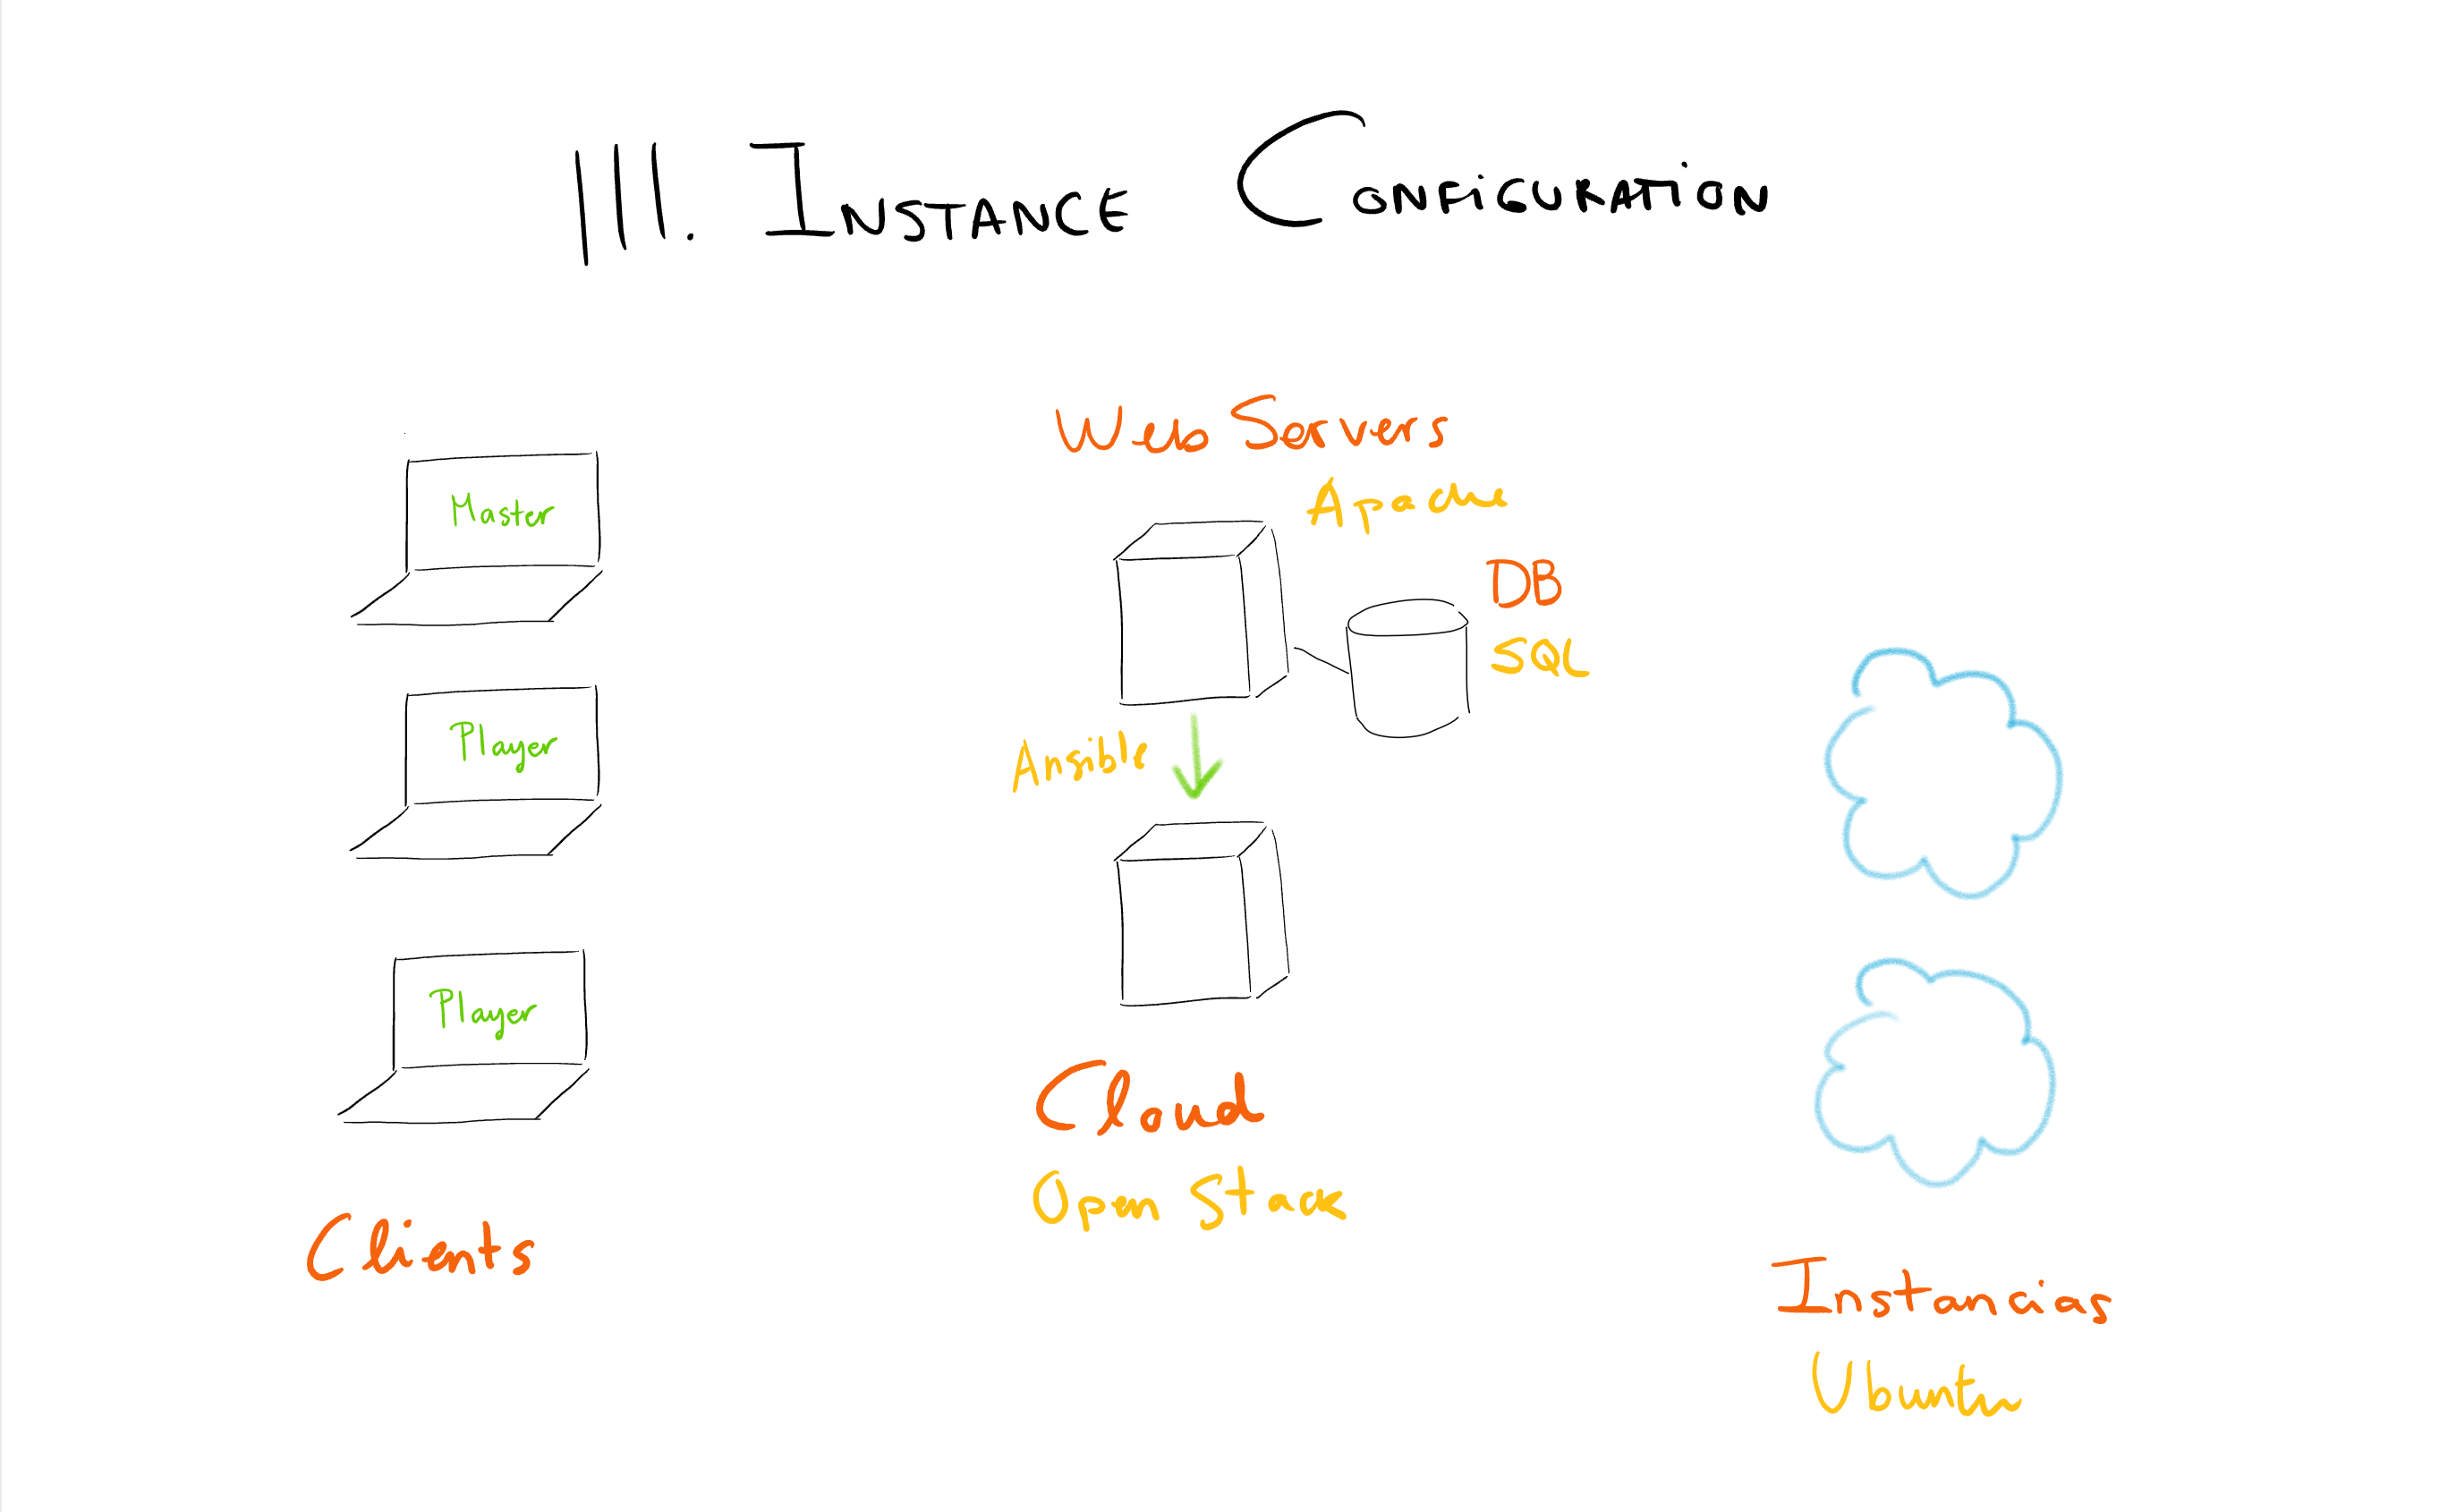
\includegraphics[width=1\textwidth]{images/Phase3.png}
\label{fig:UC3}
\end{figure}


Now, the OpenStack Cloud Server commences the deployment of the remote Cloud Campaign and returns its IP address for further communication. 
\begin{figure}[h!]
\caption{}
\centering
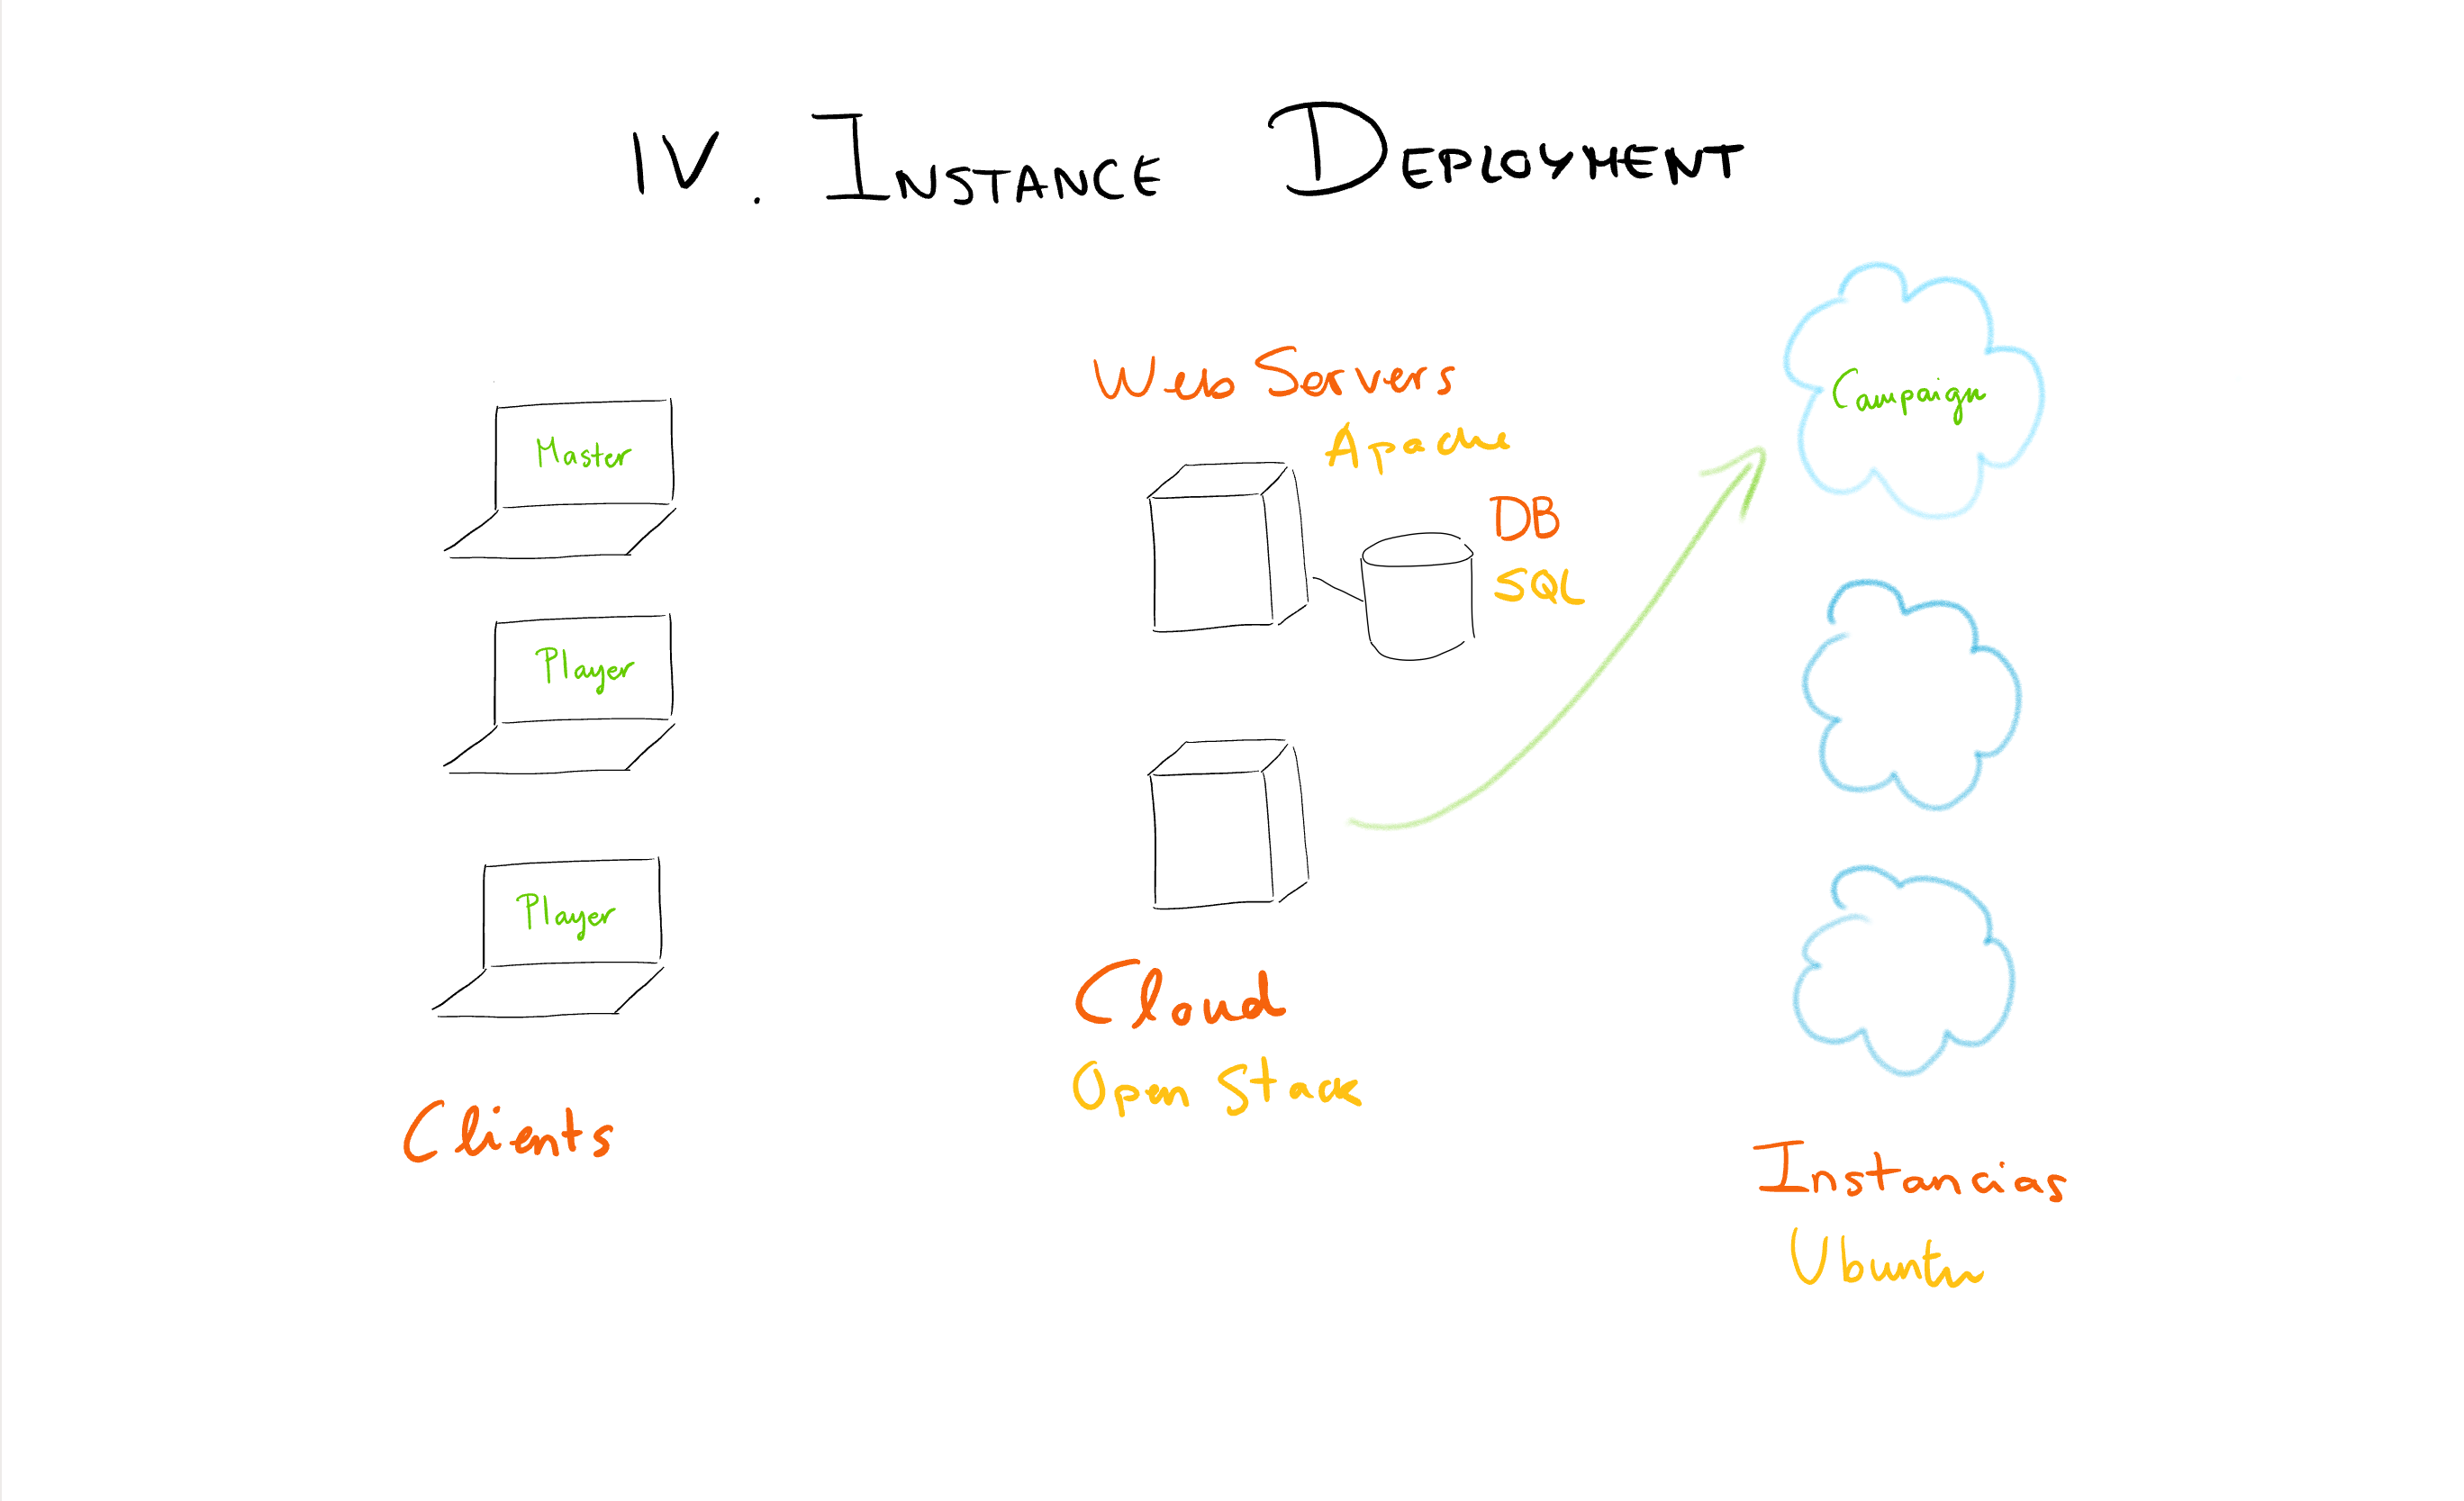
\includegraphics[width=1\textwidth]{images/Phase4.png}
\label{fig:UC4}
\end{figure}


Using Ansible, the Web Server then configures the previously defined characters and Dungeon Master in charge of the Campaign. In this instance, such characters will have the users and groups configured, as well as the corresponding Spell files and Access Control Lists for each of them. [\autoref{fig:UC4}]

\begin{figure}[h!]
\caption{}
\centering
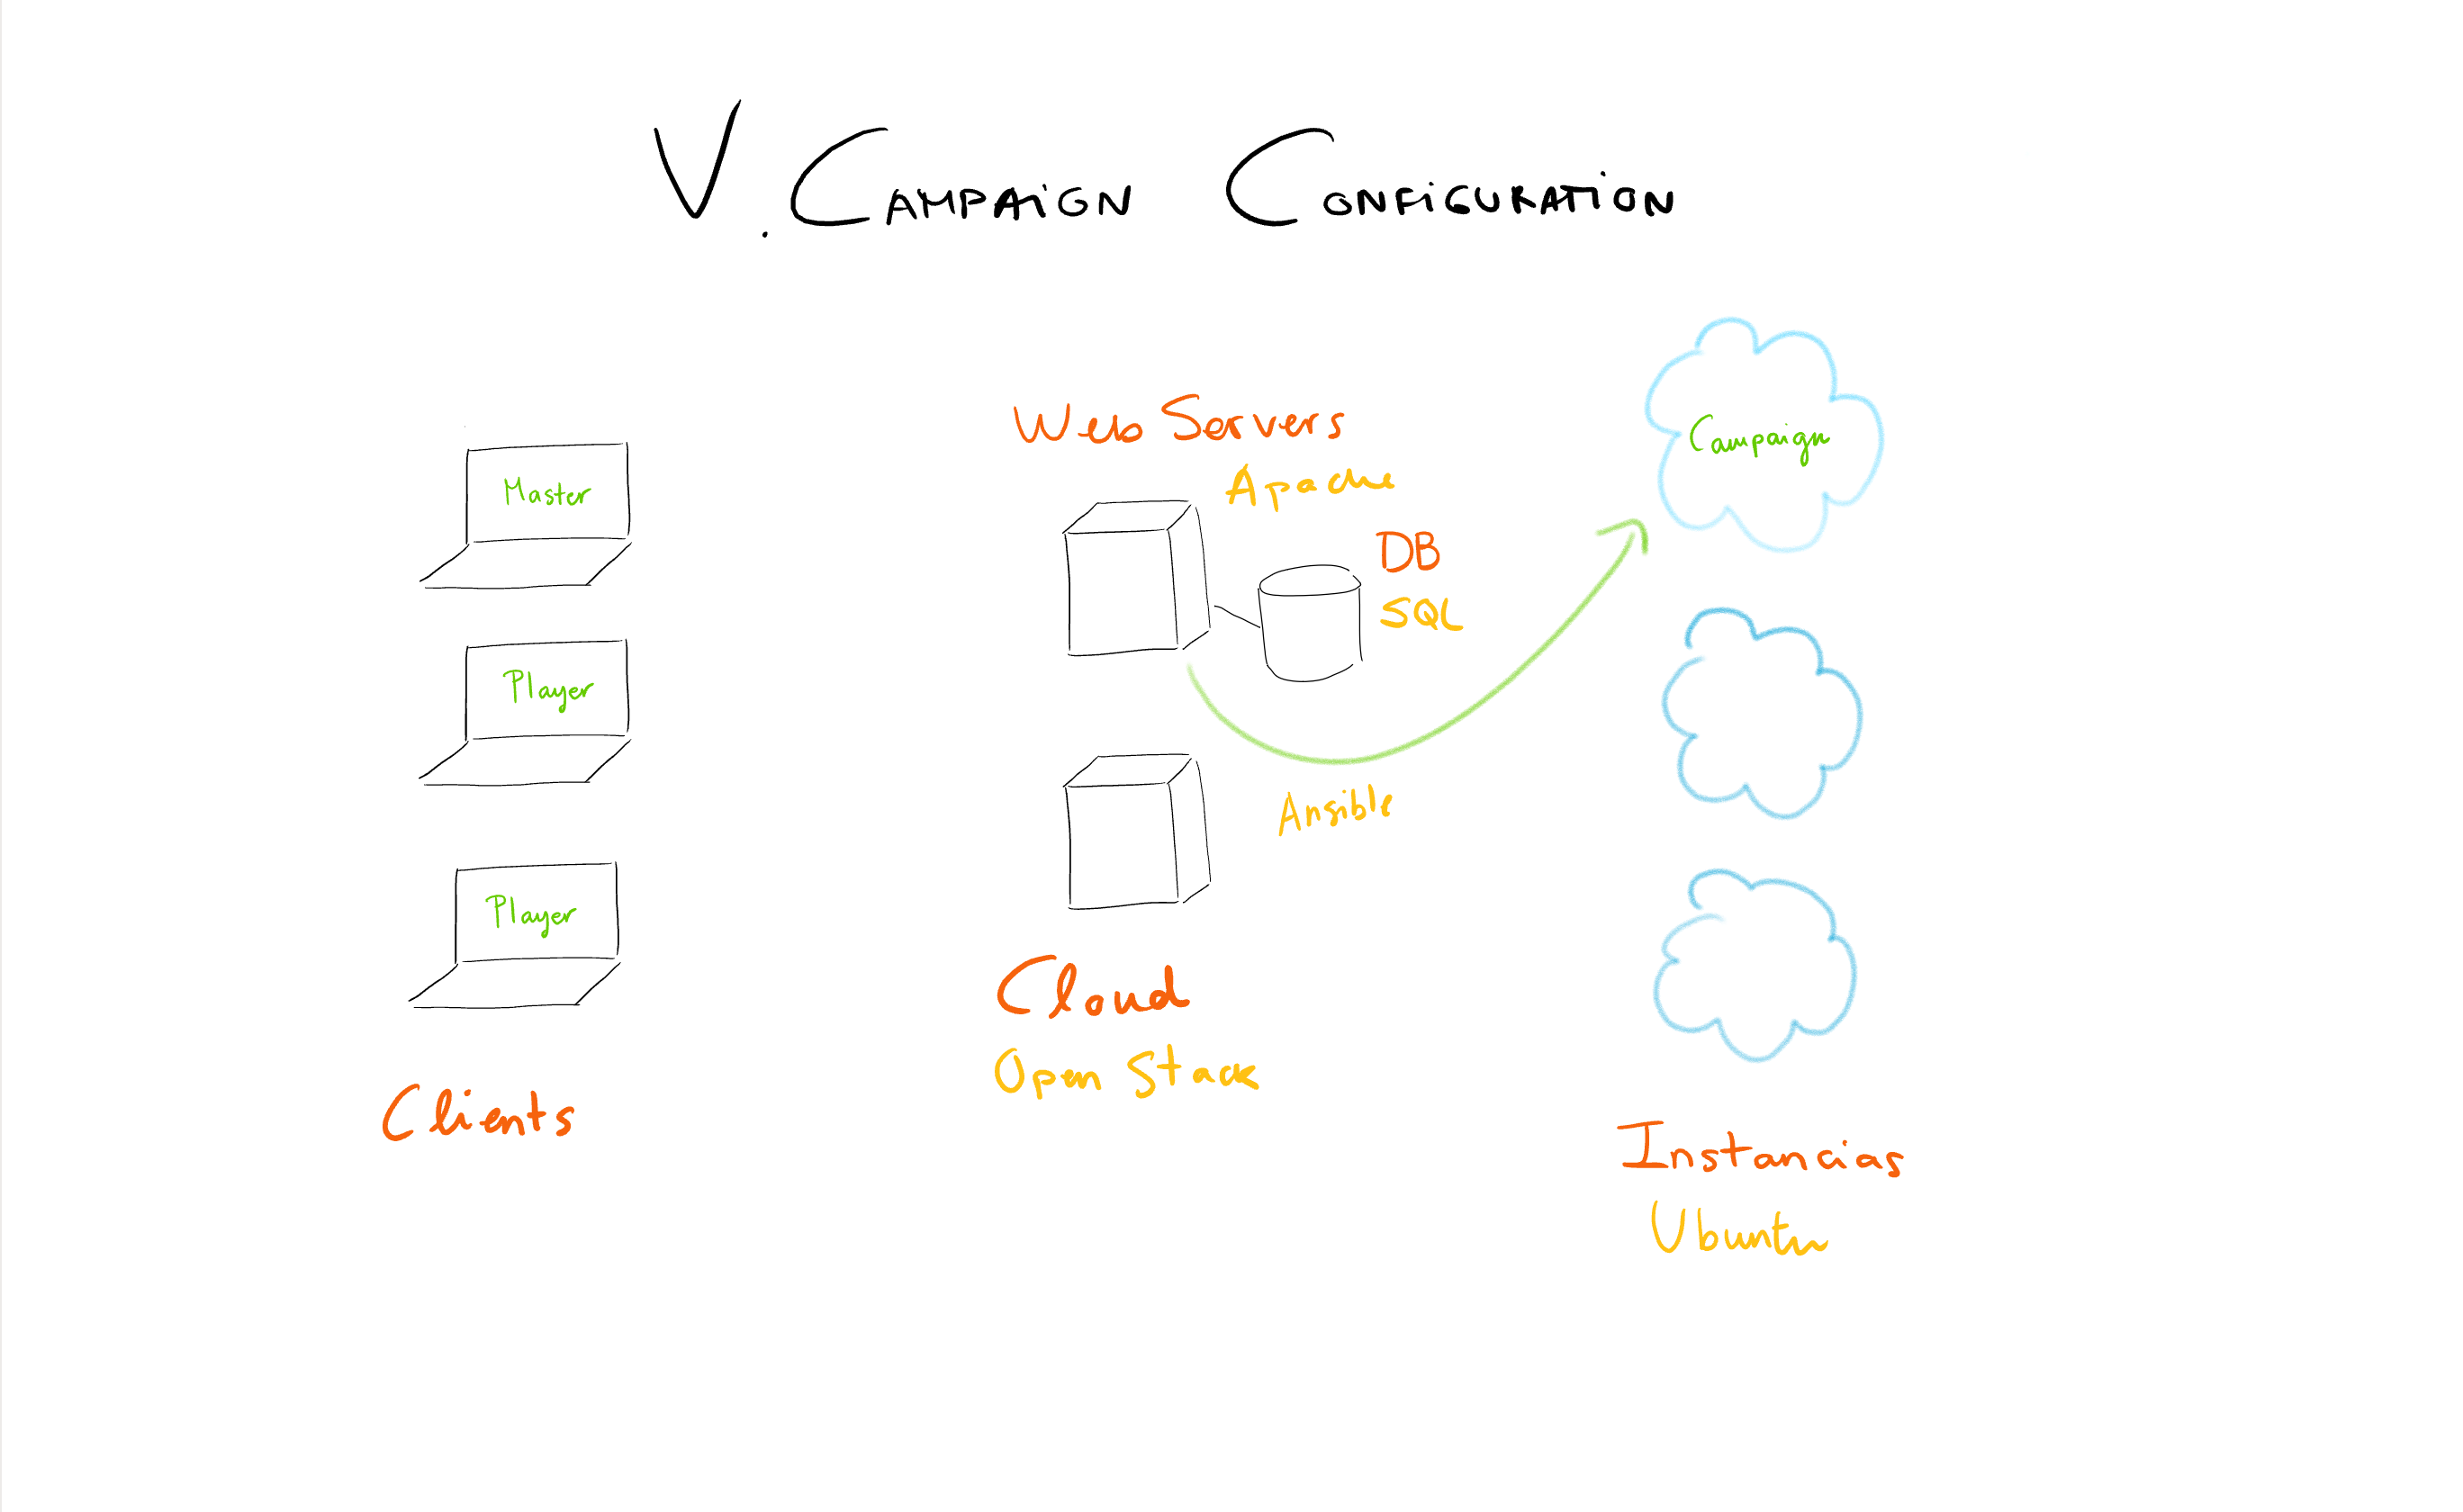
\includegraphics[width=1\textwidth]{images/Phase5.png}
\label{fig:UC5}
\end{figure}


With the Cloud Campaigns in place and ready to go, the service users can now freely connect to the instances through SSH connections and start playing and enjoy their newly created Campaign platform.

\begin{figure}[h!]
\caption{}
\centering
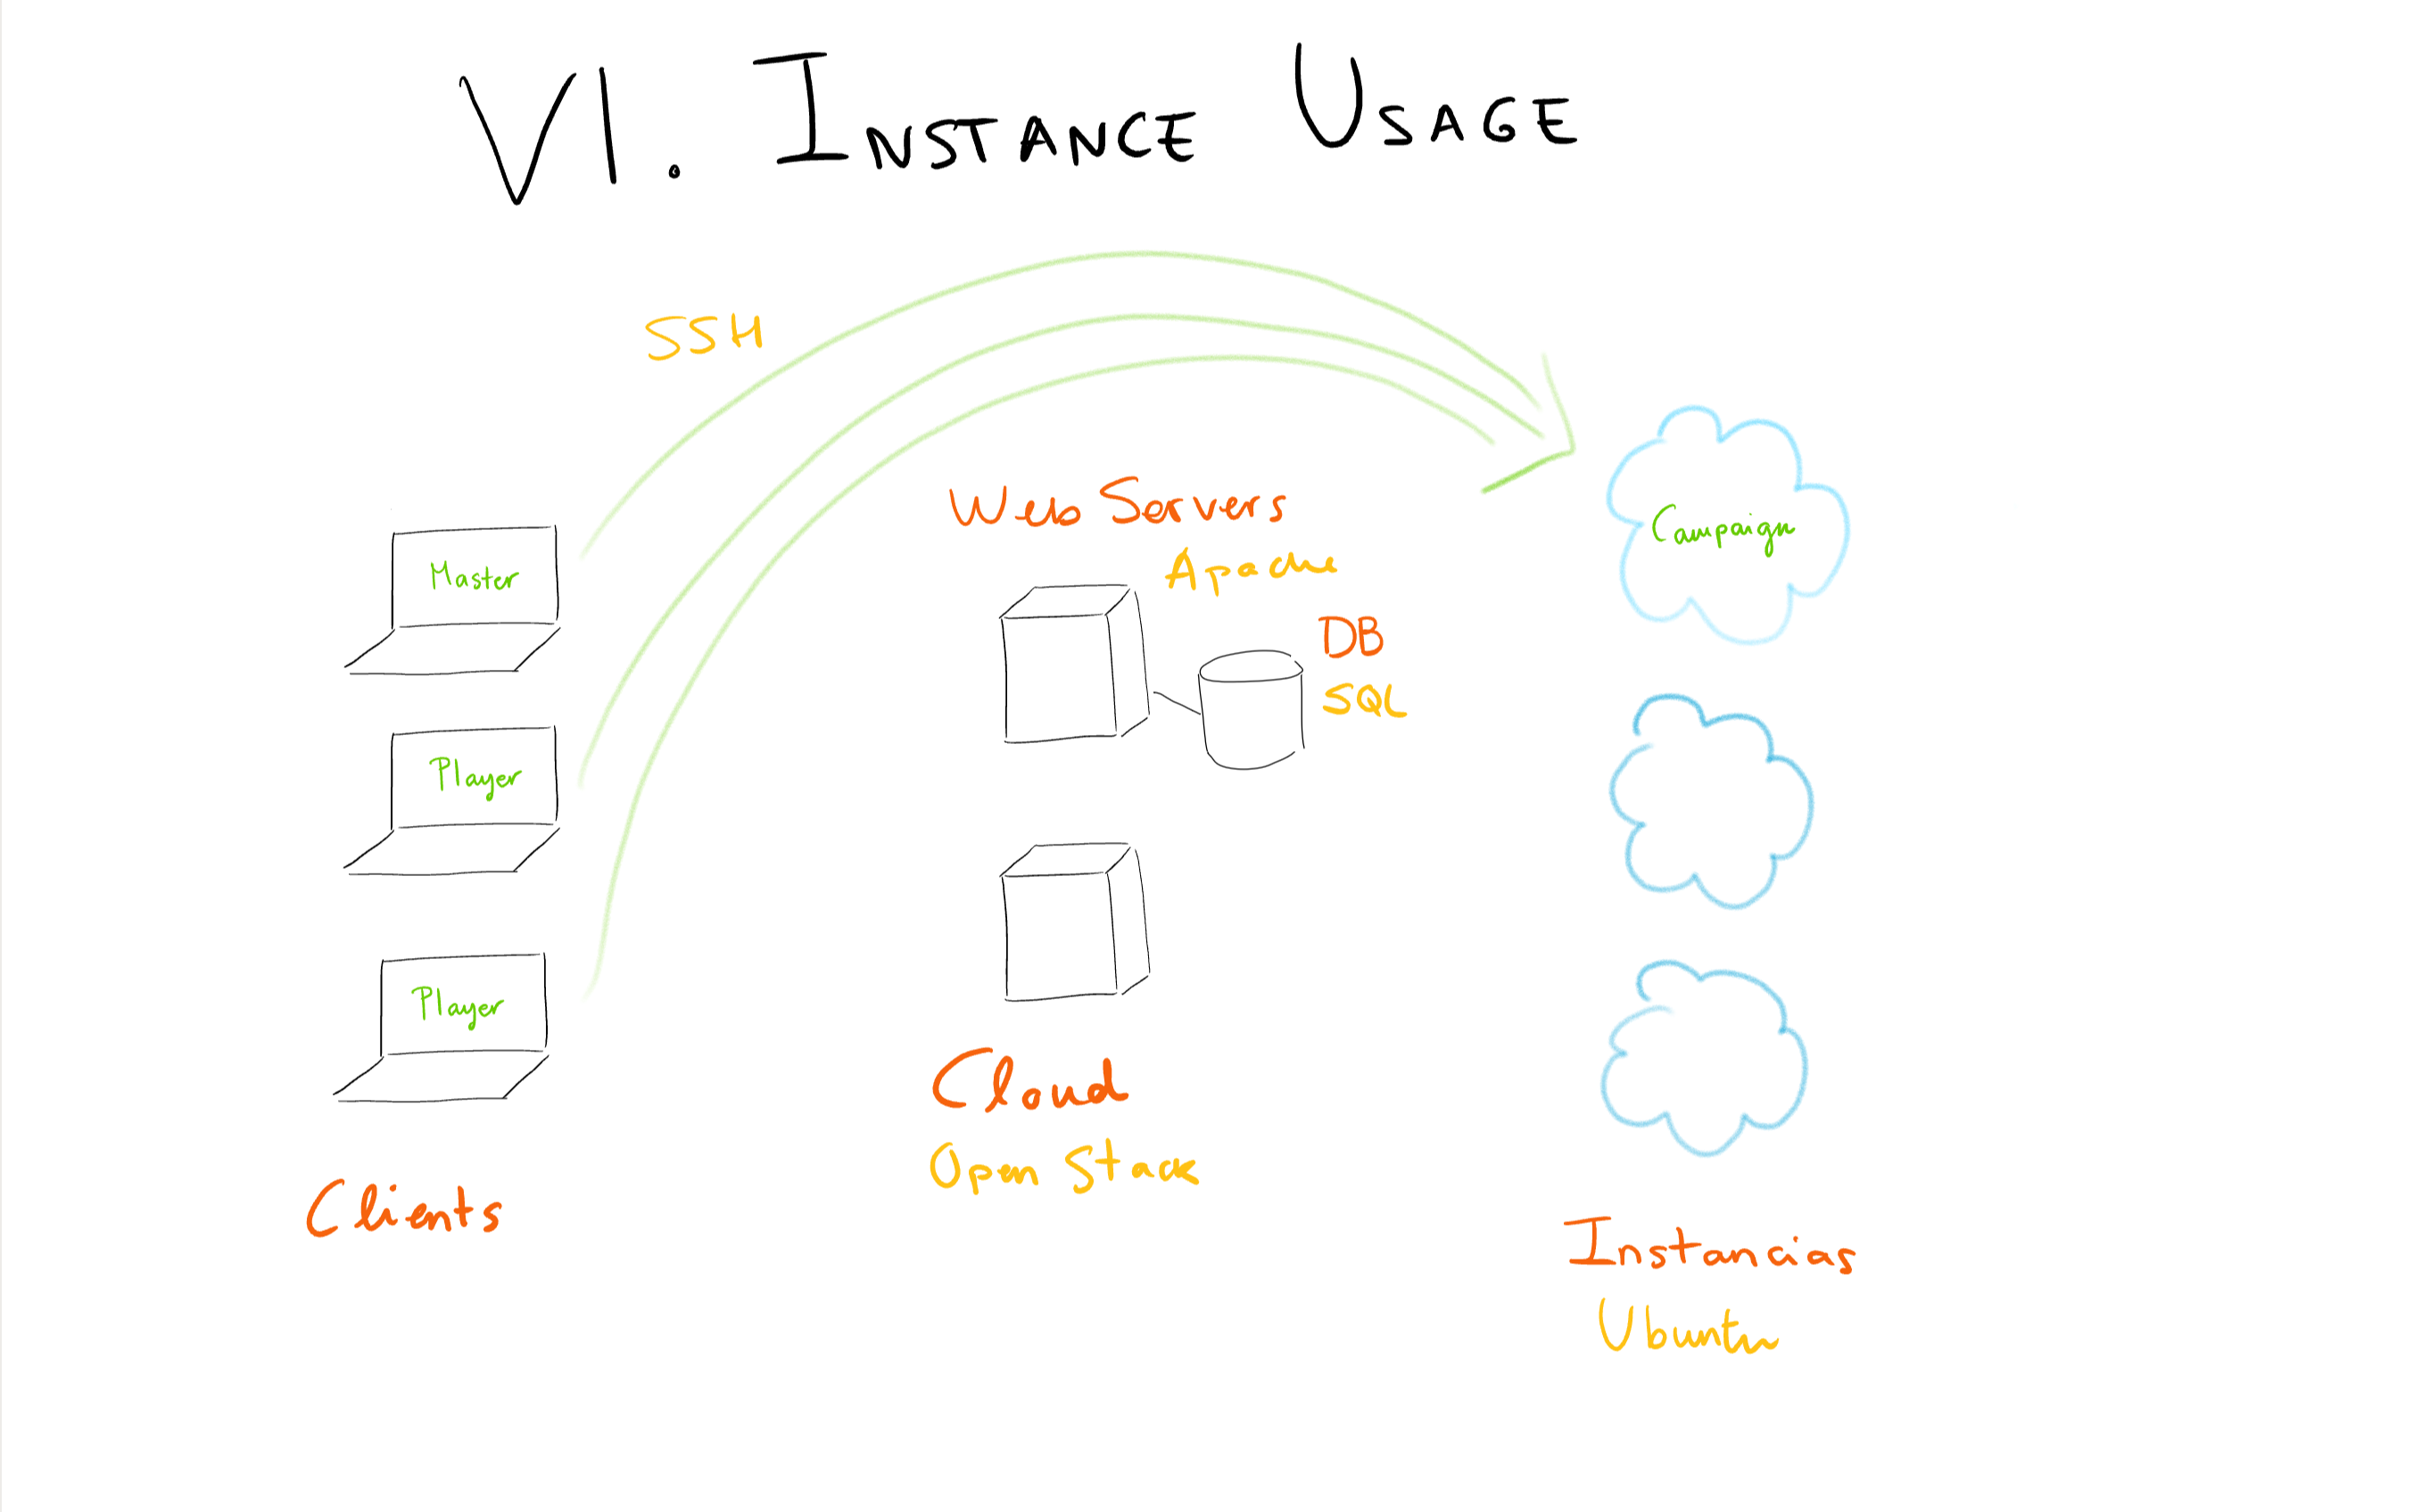
\includegraphics[width=1\textwidth]{images/Phase6.png}
\label{fig:UC6}
\end{figure}


Through Ansible, we have set up a flexible maintenance system to remotely carry out maintenance tasks in the instances. For now, it performs flexible system updates to keep the Campaigns with state-of-the-art security capabilities at all times. [\autoref{fig:UC7}]

\begin{figure}[h!]
\caption{}
\centering
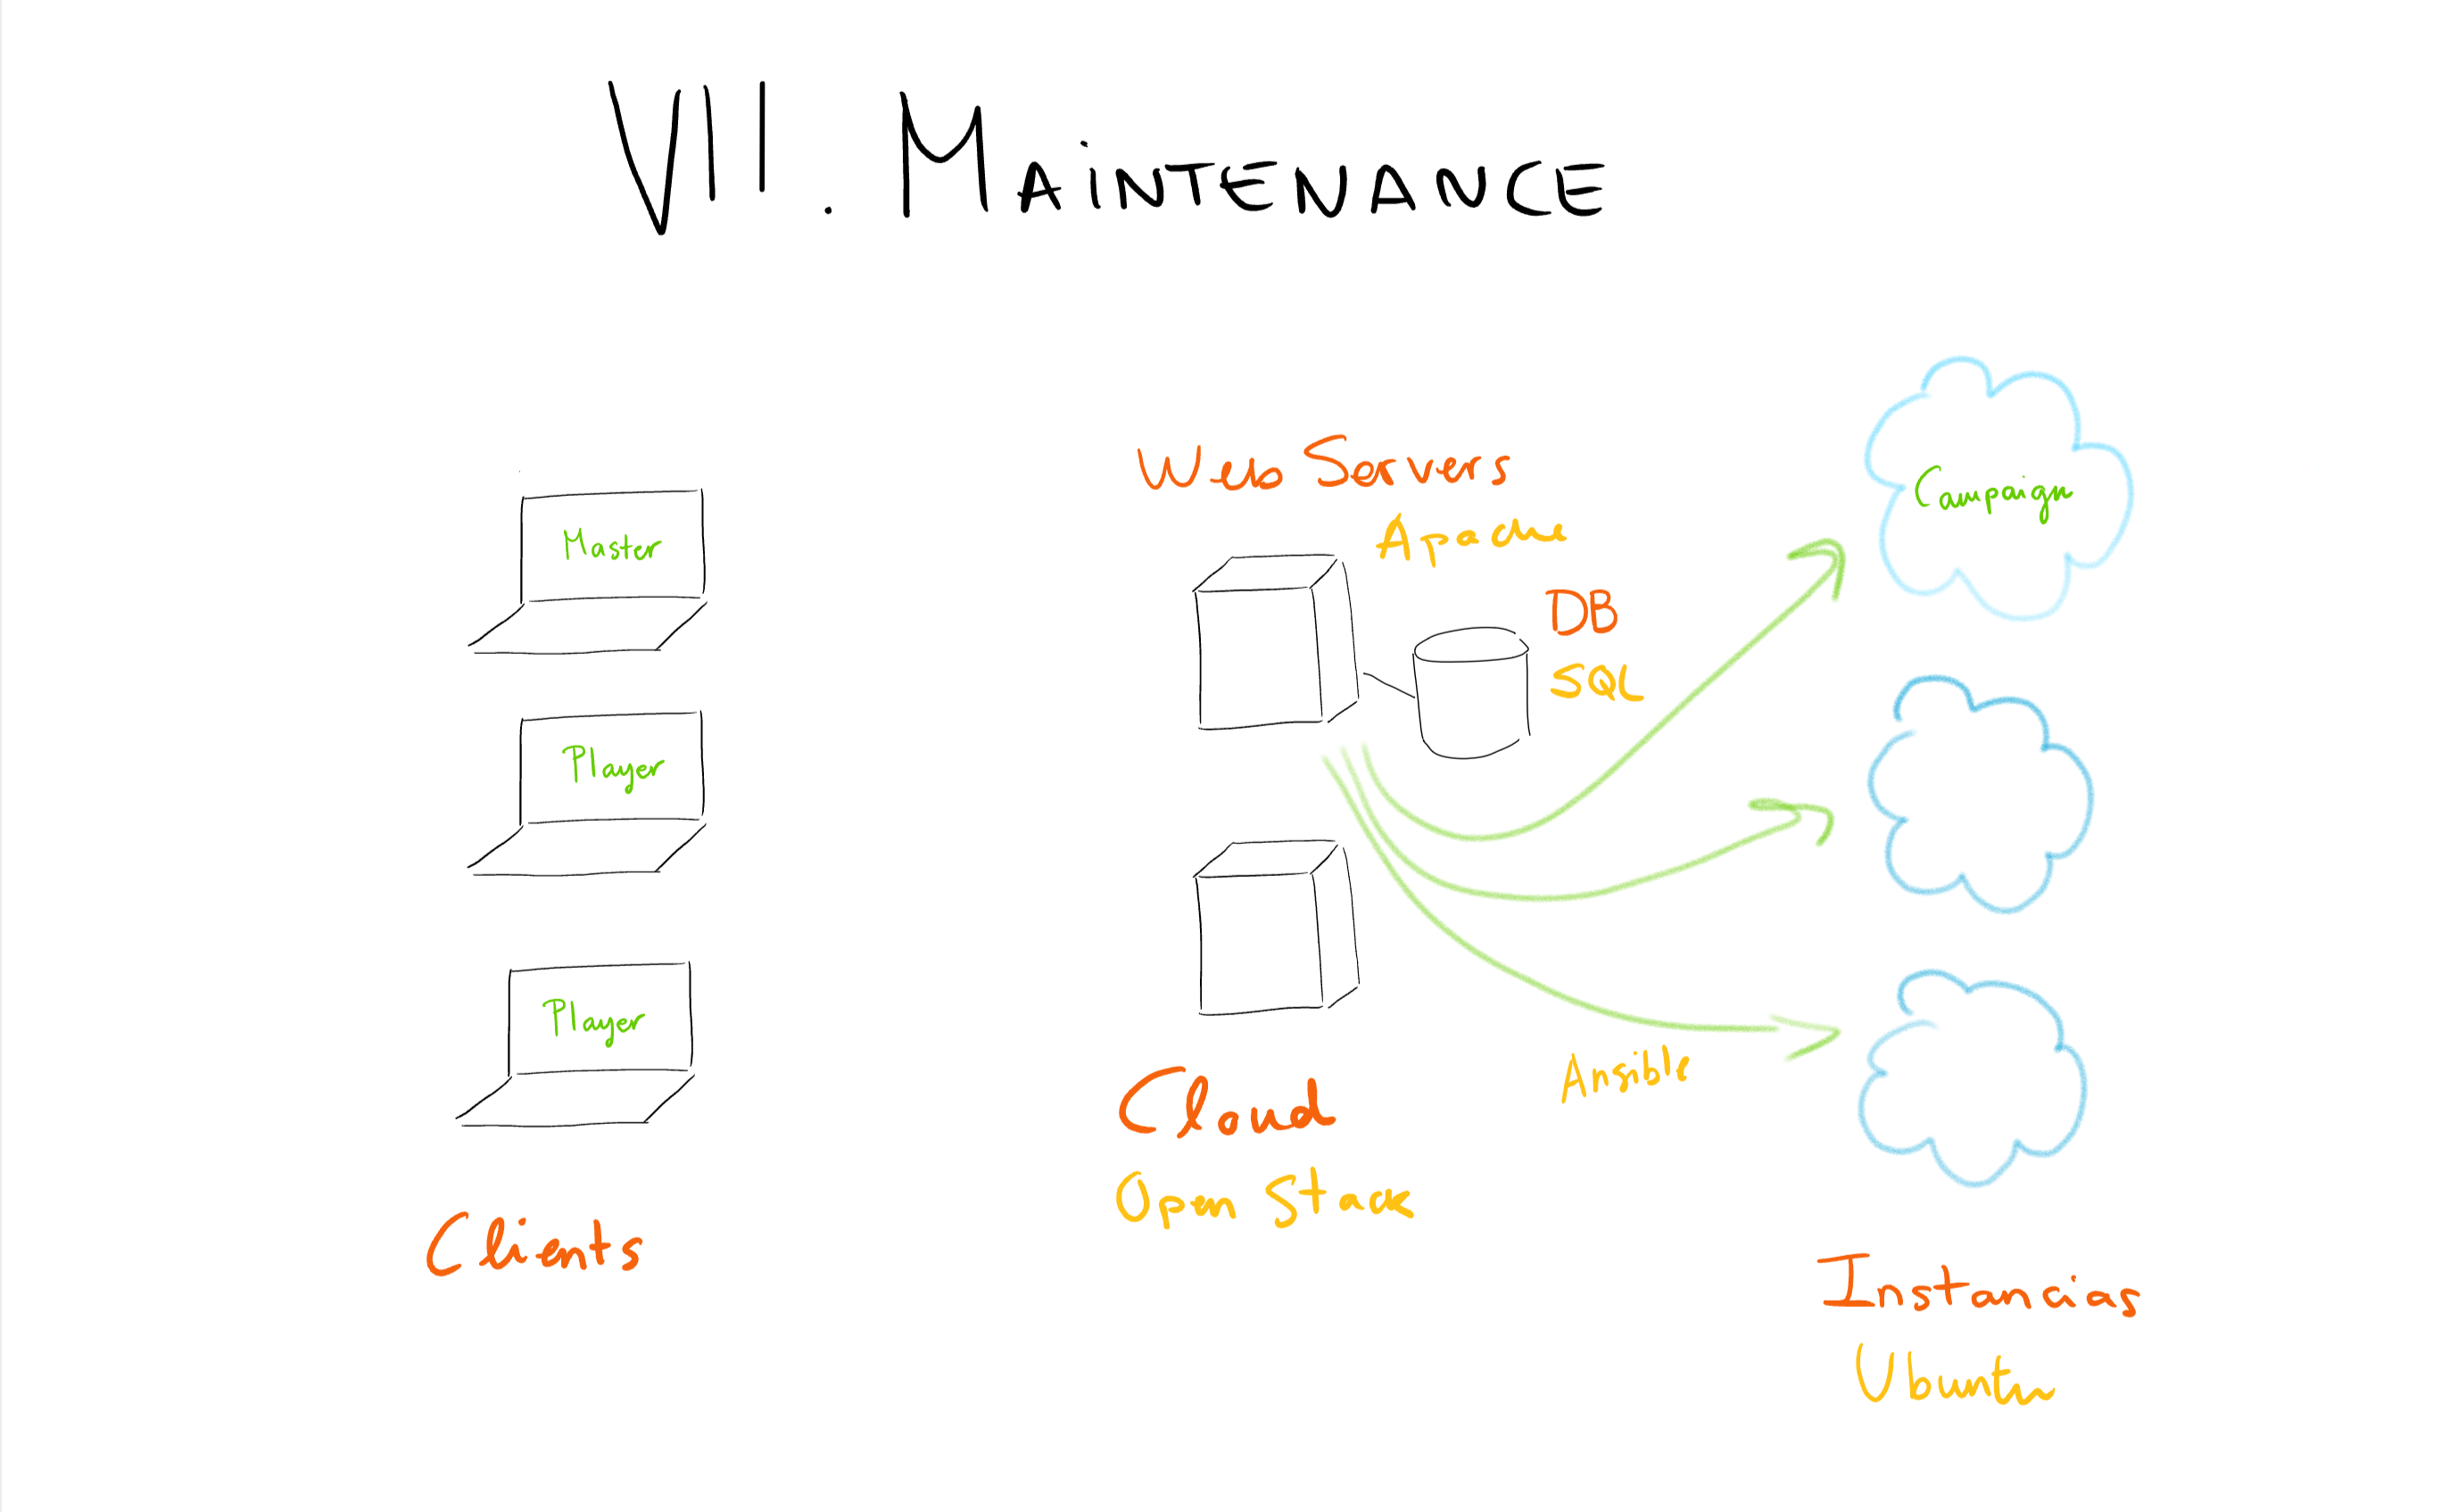
\includegraphics[width=1\textwidth]{images/Phase7.png}
\label{fig:UC7}
\end{figure}



%%%%%%
\chapter{Conclusions}
\label{ch:Conclusions}

%i am a happy chicken
%the happy chicken sometimes gets sad
%but it's still a happy chicken on the inside
%poko :>

Sometimes when playing role games, the process of creation and configuration of the campaign can become a tedious process which ends up lagging behind the moment in which to start the game itself. Through this new service, Dungeons\&Dragons as a Service, we have attempted to ease out that process, letting the user through a guided path across the creation process in which he/she can leave its creativeness roam free while worrying not about the intricacies of the spawning of the campaign. This campaign is created in a remote Cloud Server based on OpenStack, which they can connect to and play straight away. DaaS is in charge of the configuration of such instances through Ansible so the server is only left to be played in.

Our newly born service not only aids in the creation of the campaign characters but also takes charge of automating the process of controlling which abilities and spells can be accessed by who with a predefined Multi-layer security model (BLPP), which becomes transparent to the user and lets the character take control through the journey of discovery that is the Dungeons \& Dragons campaign.



\vskip 8cm

\textit{This project was created with lots of caffeine, lack of sleep over a week, a couple of teaspoons of desire to die and a pinch of freaky love.}

\textit{PD. RIP Alex, fallen in battle (either was or will be). Agur eta ohore.}


\end{document}
